\section{High Level Components}
From a high level point of view, the PowerEnJoy system is composed by four elements.

The mobile and the desktop application are included in the \textit{Client} component. The role of this component is to allow the user to be able to book and rent cars, which are the main functions of PowerEnJoy. This is possible thanks to the communication that the clients establish with the application server.

The \textit{Application} is the component in which all the logic of the system is executed. The calls to this component, coming from the clients, are routed to the dedicated controller that will be in charge to execute them.

The application level is stateless. For this reason a \textit{Database} is needed to store all the information about the state of the service.

The \textit{Onboard Computer} is the system component that allow all the communication about the car, between the car itself and the application level.

\begin{figure}[H]
	\centering
	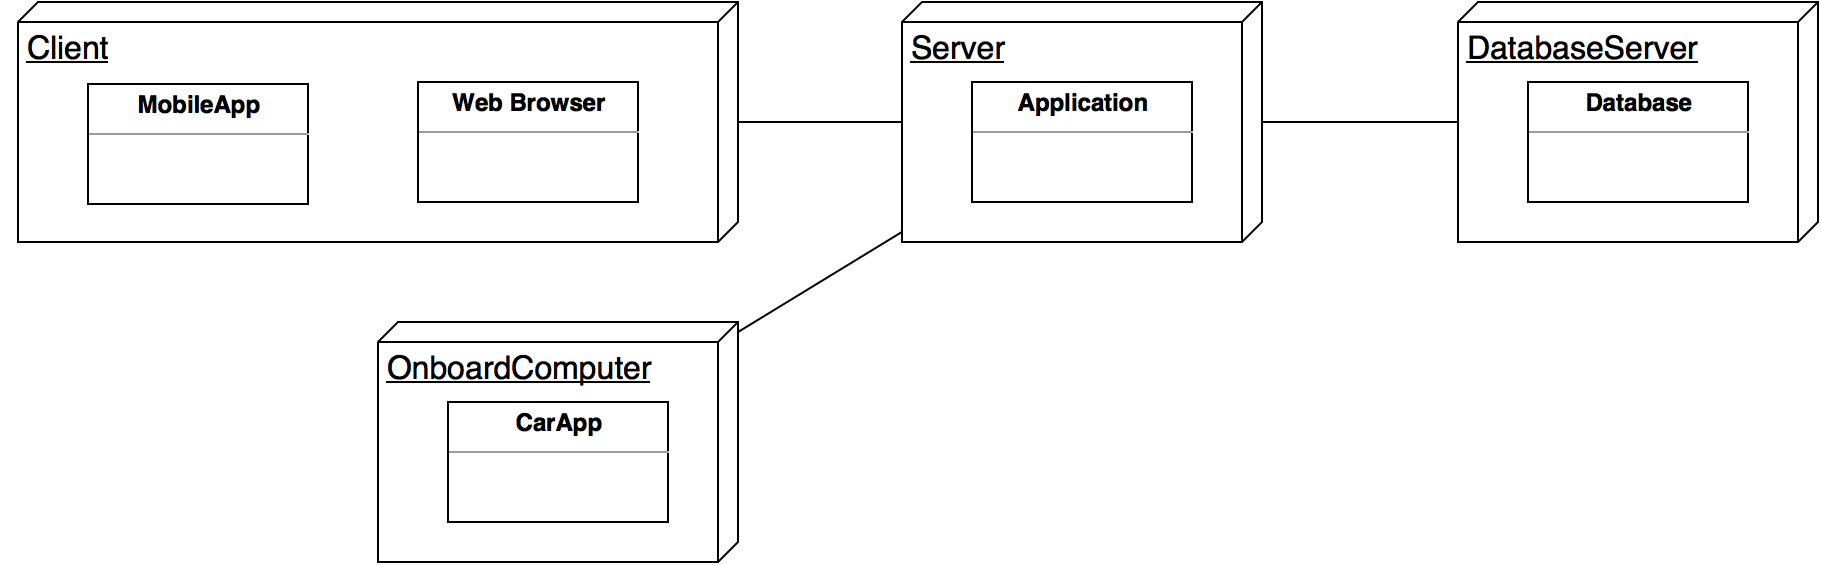
\includegraphics[width=\textwidth]{high-level-components}
	\caption[High Level Components]{The picture above represents the high level model of the PowerEnJoy system infrastructure.}
	\label{fig:high-level-components}
\end{figure}
